\documentclass[a4paper,12pt]{article}
\usepackage[utf8]{inputenc}
\usepackage[russian]{babel}
\usepackage{amsmath}
\usepackage{amssymb}
\usepackage{enumitem}
\usepackage{graphicx}
\usepackage{hyperref}
\usepackage[a4paper, top= 1cm, bottom=2cm, left=2cm, right=2cm]{geometry}

\hypersetup{
    colorlinks=true,
    linkcolor=blue,
    urlcolor=blue, 
}

\title{Площади}

\begin{document}
\maketitle
    \subsection*{Задачи}
    \begin{enumerate}
        \item Докажите, что  $S_ {\Delta ABC}$ $ \leq AB \cdot BC/2$.
        \item Основание треугольника на 4 меньше высоты, а площадь треугольника равна 96. Найдите основание и высоту треугольника. 
        \item Докажите, что медианы разбивают треугольник на шесть равновеликих треугольников.
        \item Листок календаря частично закрыт предыдущим оторванным листком (см. рисунок). Вершины A и B верхнего листка лежат на сторонах нижнего листка. Четвёртая вершина нижнего листка не видна  — она закрыта верхним листком. Верхний и нижний листки, естественно, равны между собой. Какая часть нижнего листка больше  — закрытая или открытая?
        \begin{figure}[h]
            \centering
            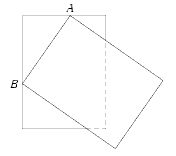
\includegraphics[width=0.25\linewidth]{image1.png}
        \end{figure}
        \item Прямоугольник разделён двумя вертикальными и двумя горизонтальными отрезками на девять прямоугольных частей. Площади некоторых из получившихся частей указаны на рисунке. Найдите площадь верхней правой части.
        \begin{figure}[h]
                        \centering
            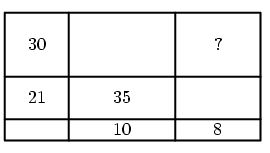
\includegraphics[width=0.25\linewidth]{image.png}
        \end{figure}
                
    \end{enumerate}
\end{document}
